\subsection{Interfaces}

Las siguientes figuras muestran las interfaces de usuario de la aplicación móvil
TreeBar, las cuales fueron diseñadas para brindar una experiencia intuitiva y
amigable al usuario final. Cada pantalla está orientada a facilitar la
navegación y el acceso a la información relevante sobre los productos y
servicios ofrecidos.

\begin{figure}[H]
    \centering
    \fbox{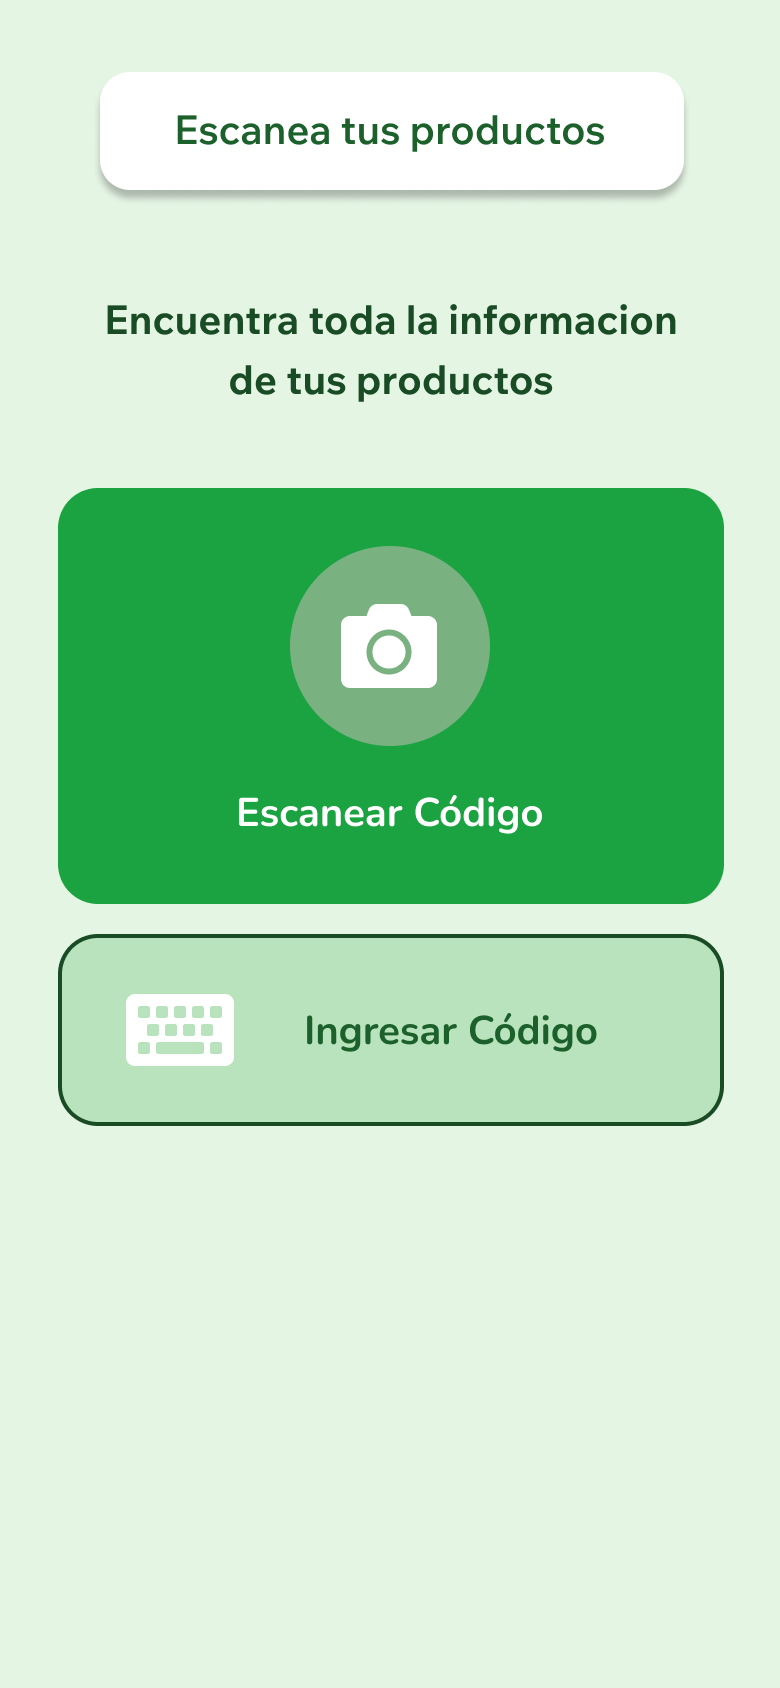
\includegraphics[width=0.5\textwidth]{imagenes/pantalla-principal.png}}
    \caption{Pantalla principal.}\label{fig:pantalla-principal}
\end{figure}

\begin{figure}[H]
    \centering
    \fbox{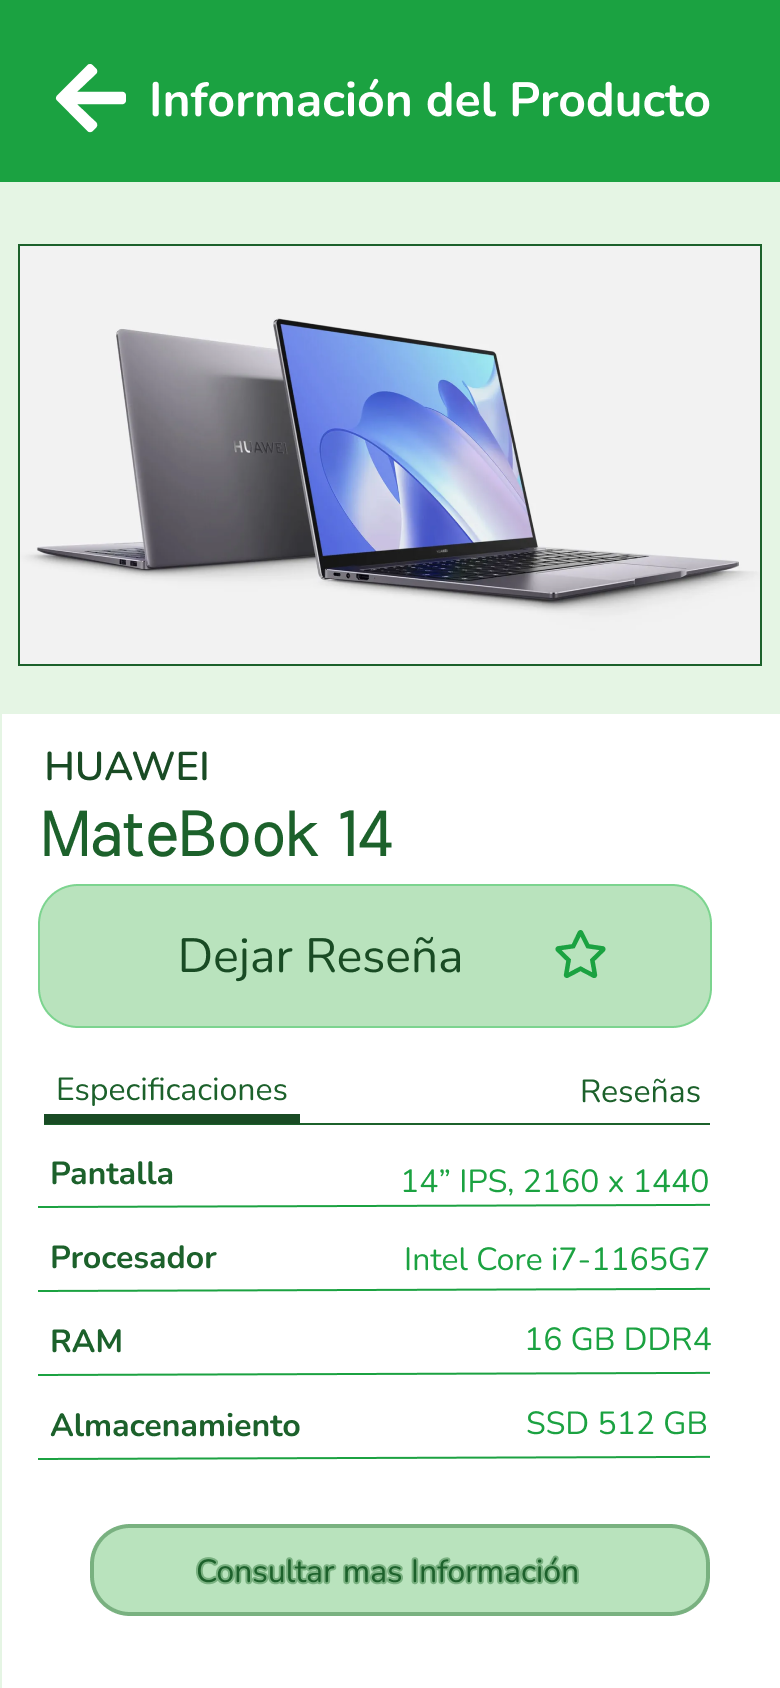
\includegraphics[width=0.5\textwidth]{imagenes/pantalla-especificaciones.png}}
    \caption{Especificaciones del producto.}\label{fig:pantalla-especificaciones}
\end{figure}

\begin{figure}[H]
    \centering
    \fbox{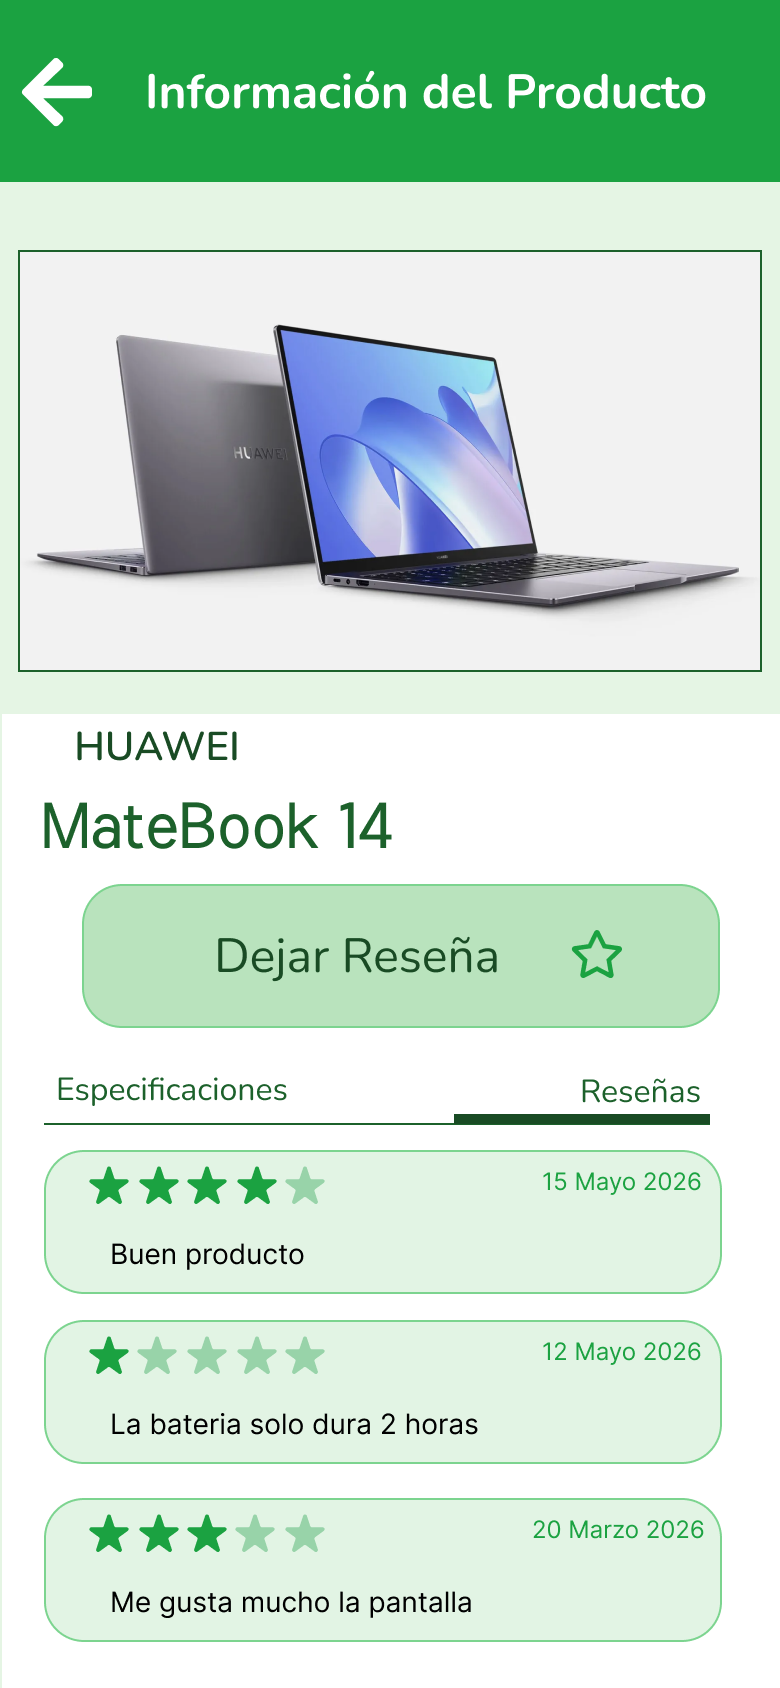
\includegraphics[width=0.5\textwidth]{imagenes/pantalla-reseñas.png}}
    \caption{Reseñas del producto por otros usuarios.}\label{fig:pantalla-reseñas}
\end{figure}

\begin{figure}[H]
    \centering
    \fbox{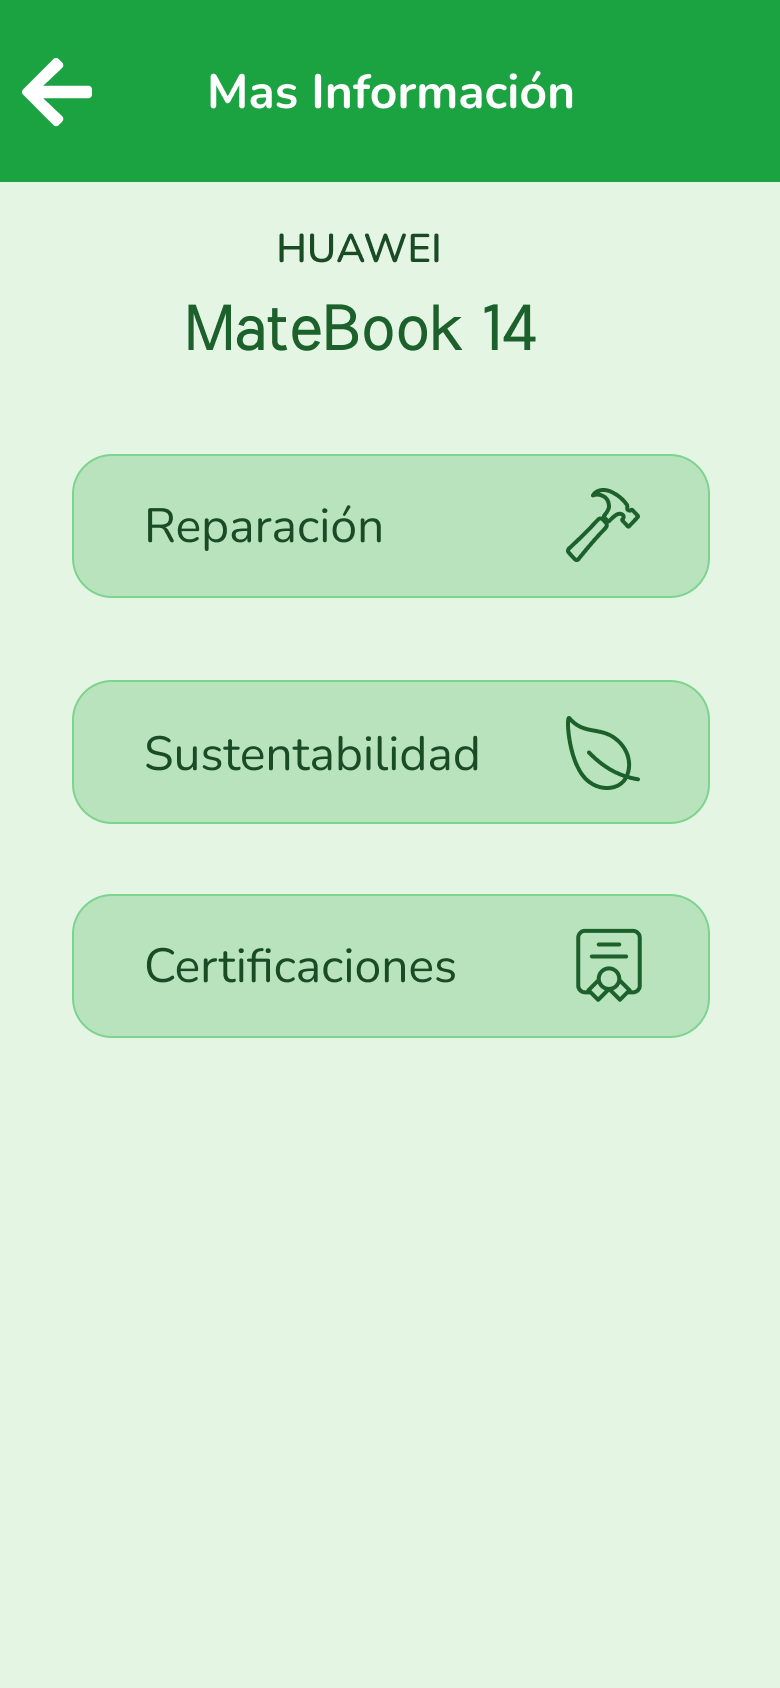
\includegraphics[width=0.5\textwidth]{imagenes/pantalla-mas.png}}
    \caption{Consultar más información sobre el producto.}\label{fig:pantalla-mas}
\end{figure}

\begin{figure}[H]
    \centering
    \fbox{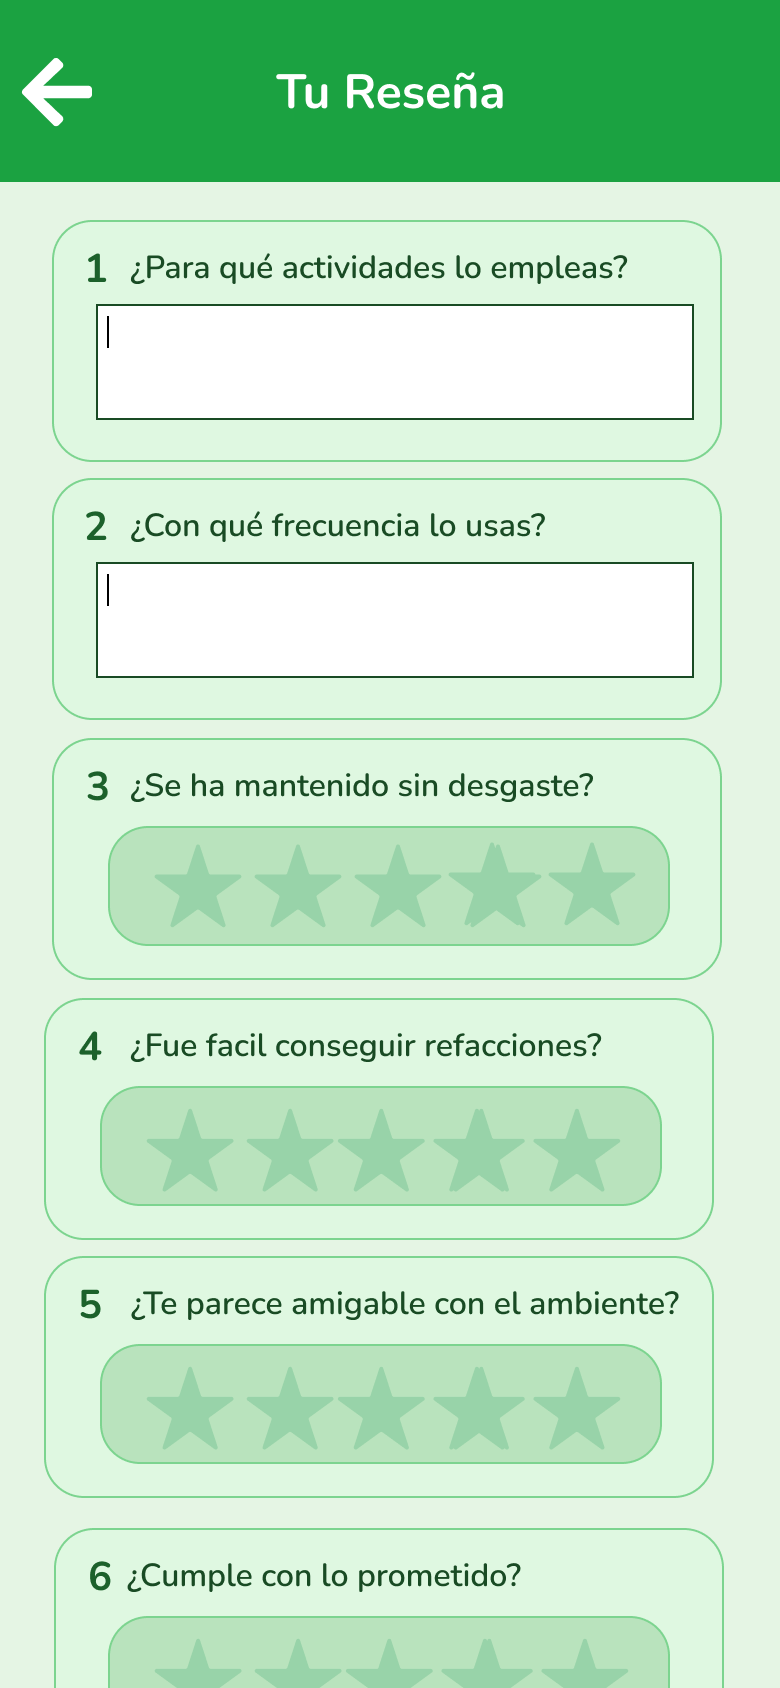
\includegraphics[width=0.5\textwidth]{imagenes/pantalla-cuestionario.png}}
    \caption{Cuestionario para conocer la opinión del usuario sobre el producto
    en ciertos aspectos.}\label{fig:pantalla-cuestionario}
\end{figure}

\begin{figure}[H]
    \centering
    \fbox{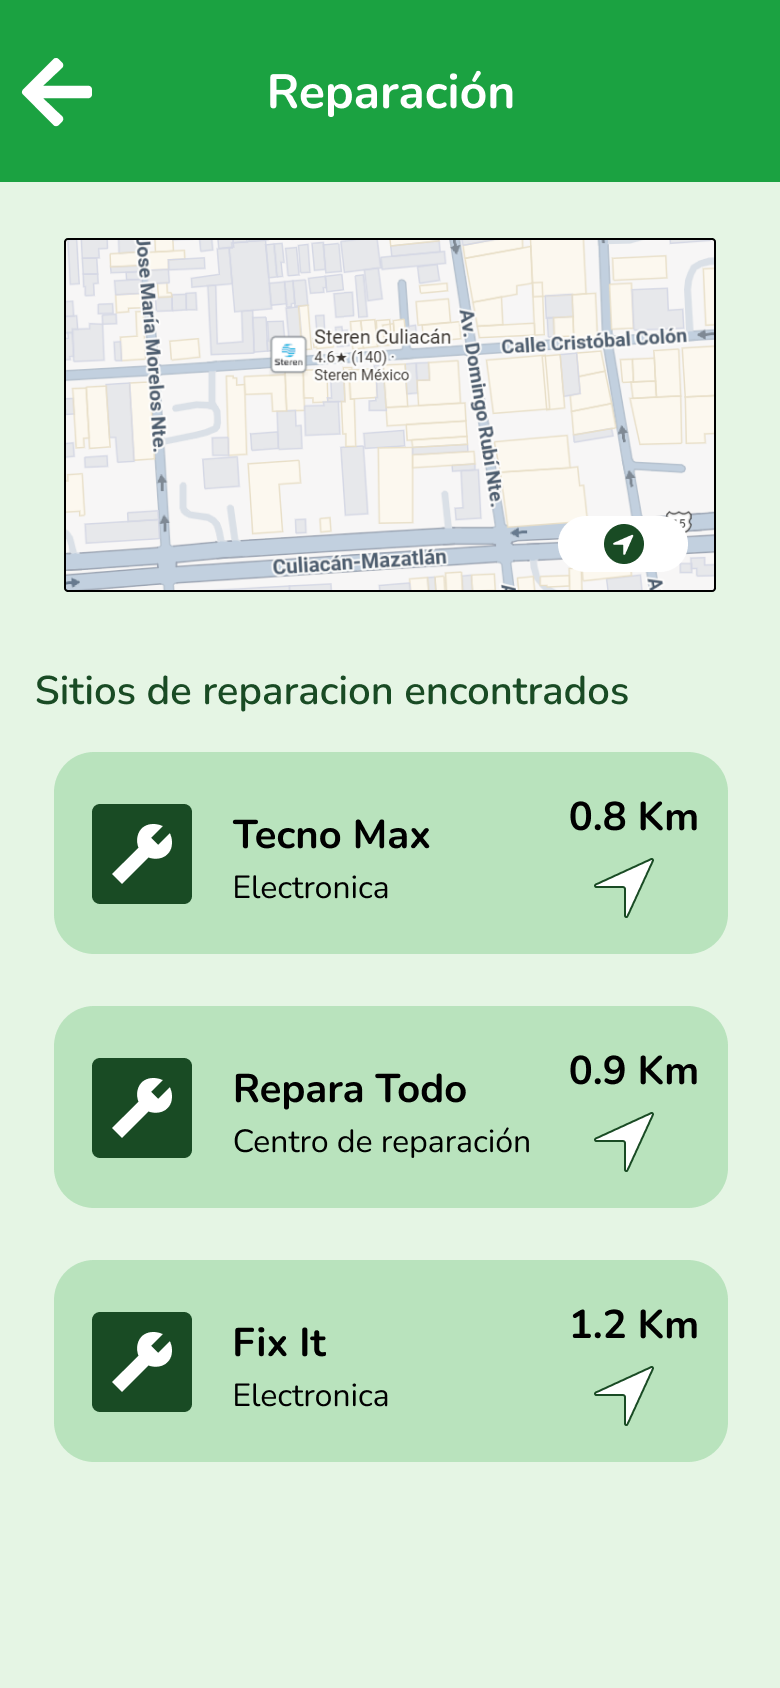
\includegraphics[width=0.5\textwidth]{imagenes/pantalla-mapa.png}}
    \caption{Mapa de sitios de reparación cercanos a la ubicación actual del
    usuario.}\label{fig:pantalla-mapa}
\end{figure}


\begin{figure}[H]
    \centering
    \fbox{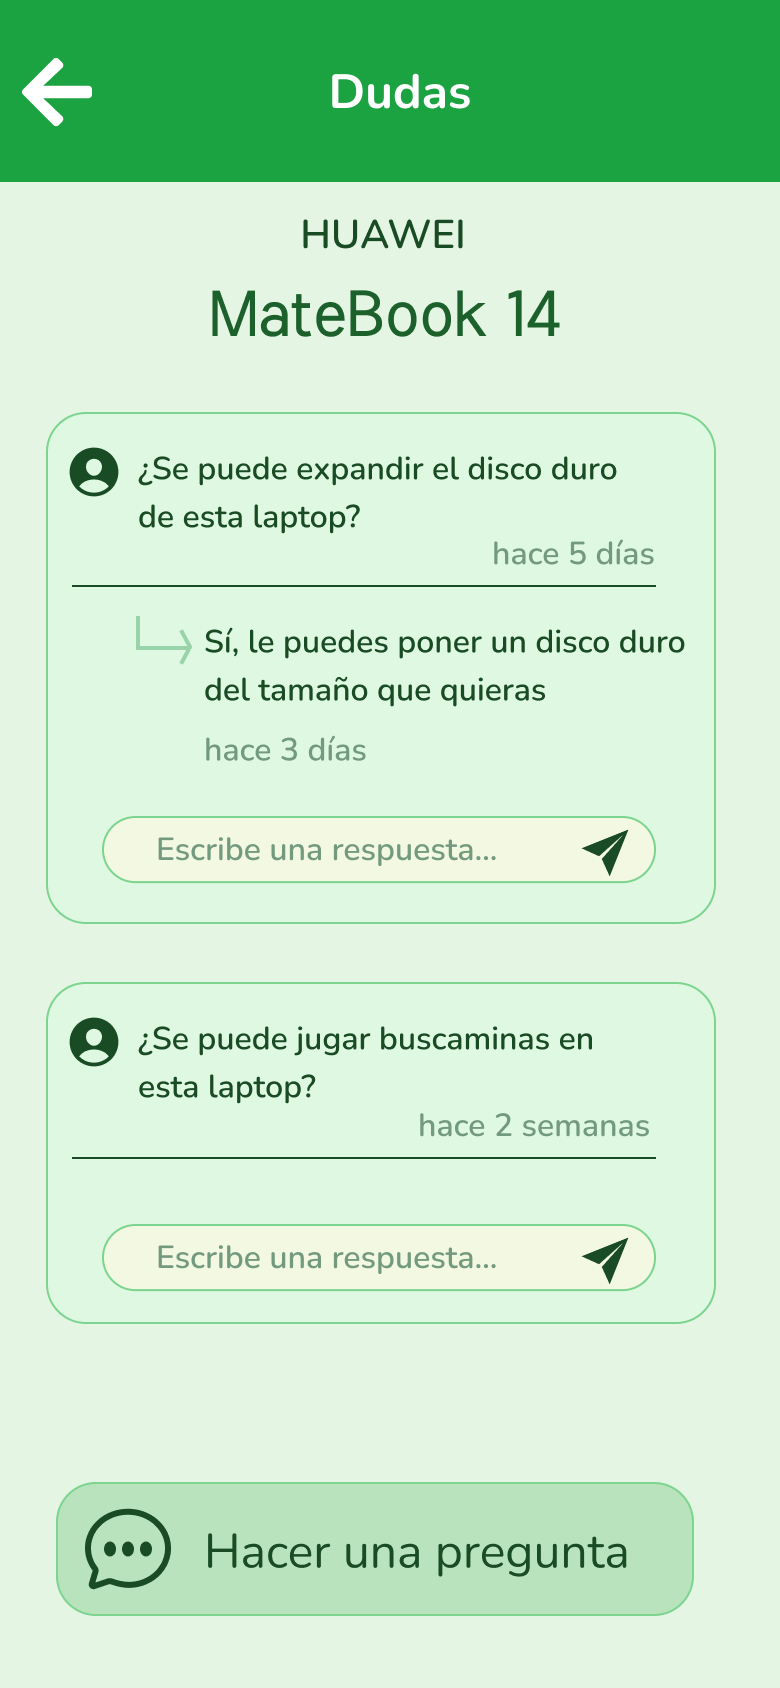
\includegraphics[width=0.5\textwidth]{imagenes/pantalla-dudas.png}}
    \caption{Pantalla de preguntas y respuestas hechas por otros
    usuarios.}\label{fig:pantalla-dudas}
\end{figure}